\begin{center}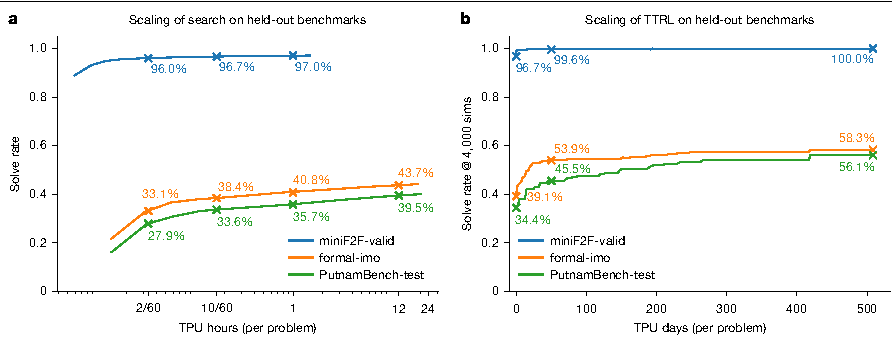
\includegraphics[width=\linewidth]{../papers/translations/alphaproof/assets/fig4.pdf}\end{center}
\phantomsection
\noindent\textbf{原文图 4. AlphaProof 表现随每题推断计算扩展.}\paperlabel{4}{alphaproof-fig4}
留出基准 miniF2F-valid、formal-imo、PutnamBench-test 的解题率. 两面板的“每题计算”均为评估 TPU 总计算除以基准题数的平均值. a, 解题率随树搜索每题计算增加的变化, 单位为 v6e TPU 小时, 对数尺度. 标出低预算, 如每题 $2/60$ TPU 小时即 1 个 TPU 用 2 分钟, 及更高预算的解题率. b, TTRL 扩展. 解题率随每目标题 TTRL 训练计算增加的变化, 单位为 v6e TPU 日, 线性尺度. 标出初步计算投入, 如 50 TPU 日或每题 50 个 TPU 用 1 日, 及 TTRL 结束的表现, 以 4,000 次模拟评估. 两面板横轴单位与尺度不同: 对数 TPU 小时与线性 TPU 日.

\noindent\textbf{图中文字对应.} Scaling of search on held-out benchmarks: 留出集上搜索扩展; Scaling of TTRL on held-out benchmarks: 留出集上 TTRL 扩展; Solve rate: 解题率; Solve rate @ 4,000 sims: 4,000 次模拟解题率; TPU hours (per problem)、TPU days (per problem): 每题 TPU 小时、每题 TPU 日. 坐标刻度、各曲线、标记与全部标注数字均保留.
